%卒論概要テンプレート ver. 3.0

\documentclass[uplatex,twocolumn,dvipdfmx]{jsarticle}
\usepackage[top=22mm,bottom=22mm,left=22mm,right=22mm]{geometry}
\setlength{\columnsep}{10mm}
\usepackage[T1]{fontenc}
\usepackage{txfonts}
\usepackage[expert,deluxe]{otf}
\usepackage[dvipdfmx,hiresbb]{graphicx}
\usepackage[dvipdfmx]{hyperref}
\usepackage{pxjahyper}
\usepackage{secdot}





%タイトルと学生番号,名前だけ編集すること
\title{\vspace{-5mm}\fontsize{14pt}{0pt}\selectfont 研究タイトル}
\author{\normalsize プロジェクトマネジメントコース 矢吹研究室 1342097 浜野太豪}
\date{}
\pagestyle{empty}
\begin{document}
\fontsize{10.5pt}{\baselineskip}\selectfont
\maketitle





%以下が本文
\section{序論}



\noindent

ドキュメントの検査にプログラムやツールによるサポートが必要である.なぜなら,システム開発の現場では,様々なドキュメントを作成する必要があるからだ.例えばプロジェクト計画書や要件定義書,マニュアルなどがある.このような文書では,読み手に誤解を与えてはいけない.さらに,わかりやすい文書を書くには一定のルールを守る必要がある.短い文で書くこと,正しい表現方法で書くこと,フォーマットを統一することなどである.このようなルールで,大量のドキュメントを人の目によってチェックすることには限界がある.

そこで継続的インテグレーションを活用する方法がある.継続的インテグレーションとは,ソフトウェア開発において,ビルドやテストを頻繁に繰り返し行なうことにより問題を早期に発見し,開発の効率化や納期の短縮を図る手法である.特に,専用のツールを用いてこのプロセスを自動化あるいは半自動化し,効率的に実施する\cite{1}.

このような継続的インテグレーションで活用されている自動化ツールを用いて,大量のドキュメントをチェックできるツールを構築する.








 



\noindent


\section{目的}
文書チェックを自動的に行うシステムを構築する.文書を提出した際に,自動で文書チェックプログラムが実行され,実行結果の表示,通知を行う.

\section{手法}
構築の手法について以下に示す.
\begin{enumerate}
\item 文書チェックプログラムの設定を行う.
\item 自動化する仮想環境に文書チェックプログラムをインストールする.
\item 自動化ツールの設定を行う.
\item 自動化ツールとGitHubの連携を行う.

\end{enumerate}

\section{結果}
Githubに課題研究の概要を提出した場合,仮想環境上の文書チェックプログラムによって自動的に文書チェックされる.
\noindent
実行結果を以下に示す.
\noindent
%図の挿入
\begin{figure}[h]
\centering
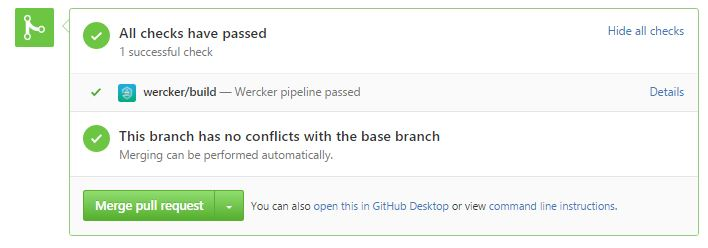
\includegraphics[width=7cm,clip]{3.JPG}
\caption{文書チェックの結果エラーがない場合}\label{}
\end{figure}
%図の挿入
\begin{figure}[h]
\centering
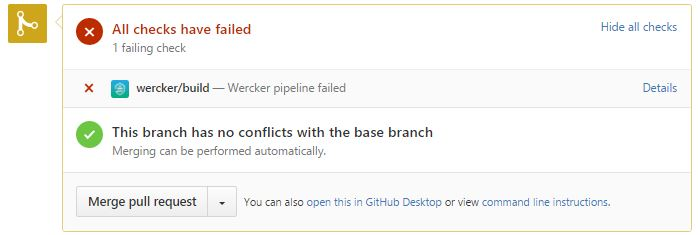
\includegraphics[width=7cm,clip]{2.JPG}
\caption{文書チェックの結果エラーがある場合}\label{}
\end{figure}

\section{考察}
仮想環境の仕様を変更することで,文書チェックプログラム以外にも自動化ができると考えた.


\section{結論}
自動的に文書チェックプログラムを行う環境を構築することができた.インフラの基礎知識や,環境構築の知識を学ぶことができた.





\bibliographystyle{junsrt}
\bibliography{biblio}%「biblio.bib」というファイルが必要.

\end{document}
